\chapter{Realizzazione del progetto}
\thispagestyle{empty}

Gli strumenti coinvolti nel progetto sono quelli descritti nei capitoli precedenti, il monocromatore Jobin-Yvon HR460 e la fotocamera intensificata 4 Picos. Di seguito si descrive il programma realizzato per il controllo dei due strumenti attraverso un unico programma.

\section{Approccio iniziale}
Avendo davanti un progetto gi� scritto e funzionante, anche se per una fotocamera diversa, il primo approccio � stato quello di cercare di integrare il vecchio programma sostituendo i subVI della fotocamera precedente con quelli della fotocamera attuale. Tale tentativo si � rivelato fin dall'inizio fallimentare in quanto il codice del vecchio progetto risulta troppo caotico e avviluppato per essere modificato senza operare ingenti cambiamenti. Si � quindi optato per una riscrittura completa del codice prendendo sempre spunto da quello gi� scritto per le parti riutilizzabili.

\section{Struttura del progetto}
\begin{figure} [h]
	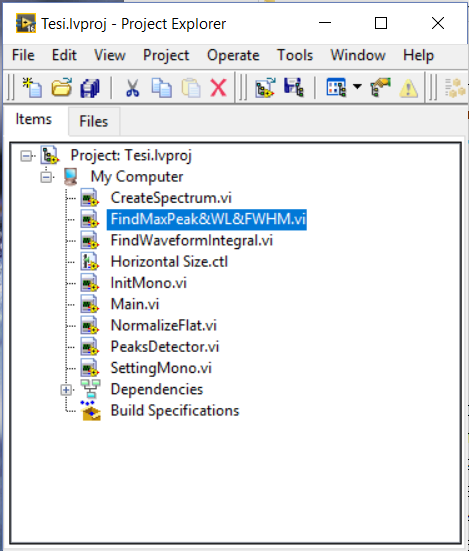
\includegraphics[width=0.5\linewidth]{img/Progetto.PNG}
	\caption{Struttura del progetto}
	\label{fig:newProj_lvproj}
\end{figure}
Per rendere il programma maggiormente organico e comprensibile si � deciso di creare un progetto LabVIEW: in questo modo i file e i subVI coinvolti sono raggruppati in un unico progetto (figura \ref{fig:newProj_lvproj}), che risulta sicuramente pi� gestibile di un semplice insieme di file.\\
Si � creato all'inizio un VI principale, un \textit{main} che ha lo stesso scopo dei \textit{main} degli altri linguaggi di programmazione. In seguito si � cercato di creare pi� subVI possibile per rendere il programma leggibile e ordinato. Si descriveranno pi� avanti i subVI contenuti nel progetto e i loro scopi.

\section{Front Panel}
\textbf{Inserire foto del front panel}
La struttura pensata per il front panel di questo progetto � quella dell'interfaccia grafica a \textit{tab} (controllo grafico di navigazione che permette all'utente di muoversi da un gruppo di controlli a un altro). Tale widget permette un'ideale suddivisione delle diverse aree di competenza del programma: di seguito verranno elencate con una descrizione degli elementi contenuti da ognuna.
\begin{itemize}
\begin{figure} [h]
	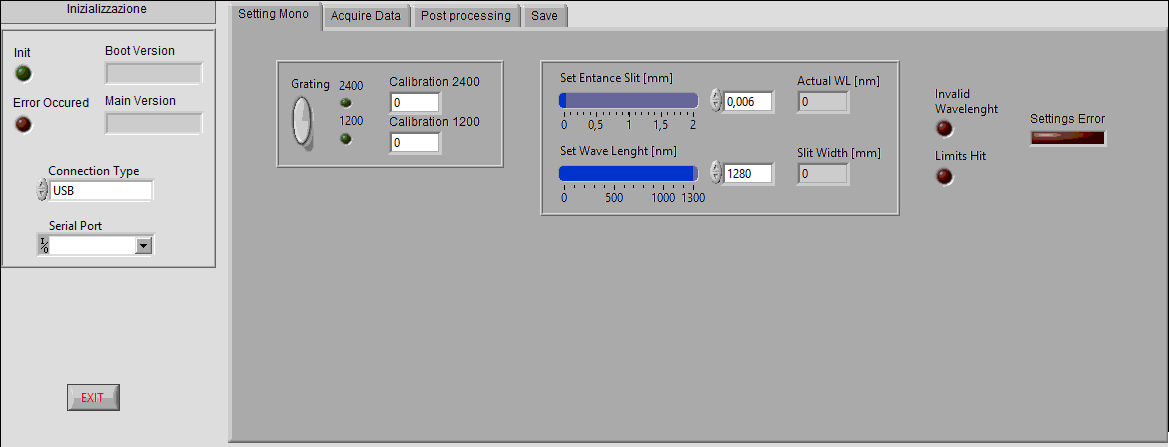
\includegraphics[width=\linewidth]{img/MainSettingMono.png}
	\caption{Front Panel del progetto, tab \textit{Setting Mono}}
	\label{fig:newProj_fp_SettingMono}
\end{figure}
	\item \textit{Setting Mono}, figura \ref{fig:newProj_fp_SettingMono}, contiene i controlli necessari al settaggio del monocromatore. \textit{Grating} per impostare il grating (1200 o 2400) e rispettivi controlli per specificarne un eventuale calibrazione. \textit{Set Entrance Slit} e \textit{Set Wave Length} per impostare la slit di entrata e la lunghezza d'onda. \textit{Actual WL} e \textit{Slit Width} per visualizzare lunghezza d'onda e slit effettivamente inserite. Sono presenti inoltre tre led: \textit{Settings Error} indica un errore generico di settaggio, \textit{Invalid Wavelength} indica l'inserimento di una lunghezza d'onda non valida e \textit{Limits hit} evidenzia l'inserimento di un valore oltre i limiti consentiti.
	\begin{figure} [h]
	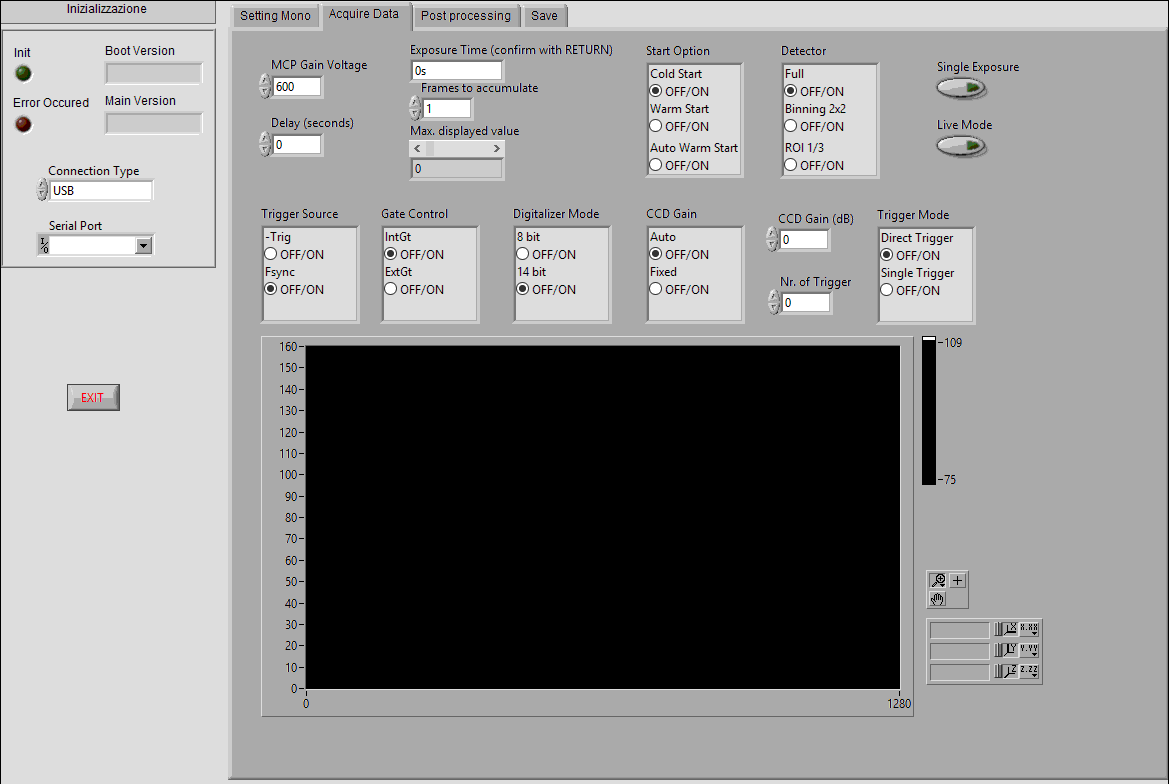
\includegraphics[width=\linewidth]{img/MainAcquireData.png}
	\caption{Front Panel del progetto, tab \textit{Acquire Data}}
	\label{fig:newProj_fp_AcquireData}
\end{figure}
	\item \textit{Acquire Data}, figura \ref{fig:newProj_fp_AcquireData}, contiene tutti i controlli per poter impostare la fotocamera e acquisire i dati.
\begin{figure} [h]
	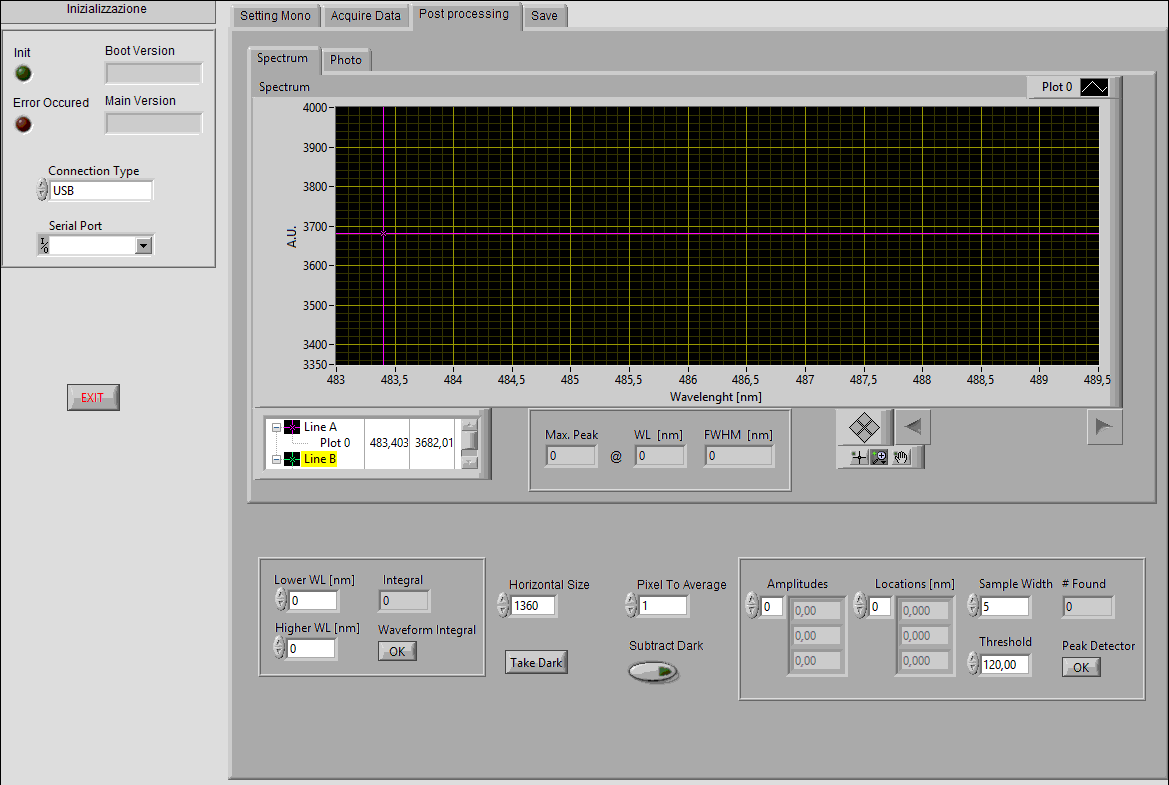
\includegraphics[width=\linewidth]{img/MainPostProc.png}
	\caption{Front Panel del progetto, tab \textit{Post Processing}}
	\label{fig:newProj_fp_PostProc}
\end{figure}
	\item \textit{Post Processing}, figura \ref{fig:newProj_fp_PostProc}, permette di visualizzare lo spettro corrispondente all'immagine acquisita ed effettuare dei calcoli su tali dati. Con \textit{Waveform Integral} � possibile calcolare l'integrale della lunghezza d'onda su un certo intervallo. \textit{Peak Detector} consente di visualizzare il numero di picchi trovati al di sopra di una certa soglia di inserire e i loro valori. Attraverso il controllo \textit{Pixel To Average} � possibile scegliere il numero di pixel da con cui fare la media da visualizzare poi nel grafico. Sono stati mantenuti anche i controlli per acquisire il background e sottrarlo alla foto.
	\begin{figure} [h]
	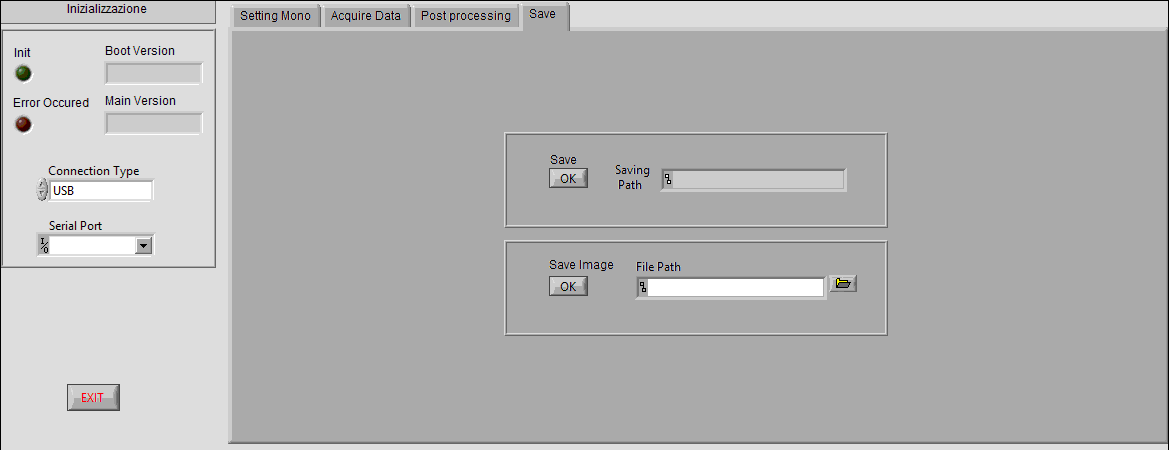
\includegraphics[width=\linewidth]{img/MainSave.png}
	\caption{Front Panel del progetto, tab \textit{Save}}
	\label{fig:newProj_fp_Save}
\end{figure}
	\item \textit{Save}, figura \ref{fig:newProj_fp_Save}, presenta due controlli booleani: \textit{Save} salva i dati be formattati in un file di testo che pu� essere aperto successivamente con altri editor, \textit{Save Image} salva invece l'immagine vera e propria.
\end{itemize}
Al di fuori di questo controllo � presente un pannello dedicato all'inizializzazione degli strumenti. Il led \textit{Init} segnala che il monocromatore � stato inizializzato senza errori e viene visulizzata anche la versione del programma, in caso contrario si attiva il led \textit{Error Occured}. Sono presenti anche due controlli per specificare la connessione che si intende utilizzare verso la fotocamera: \textit{USB} per connetterla al calcolatori attraverso cavo USB, \textit{CameraLink} o \textit{Analog} per altre modalit� di connessione non contemplate in questo progetto.\\
Infine il bottone \textit{Exit} consente di arrestare il programma nel modo corretto.

\section{Block Diagram}
\begin{figure} [h]
	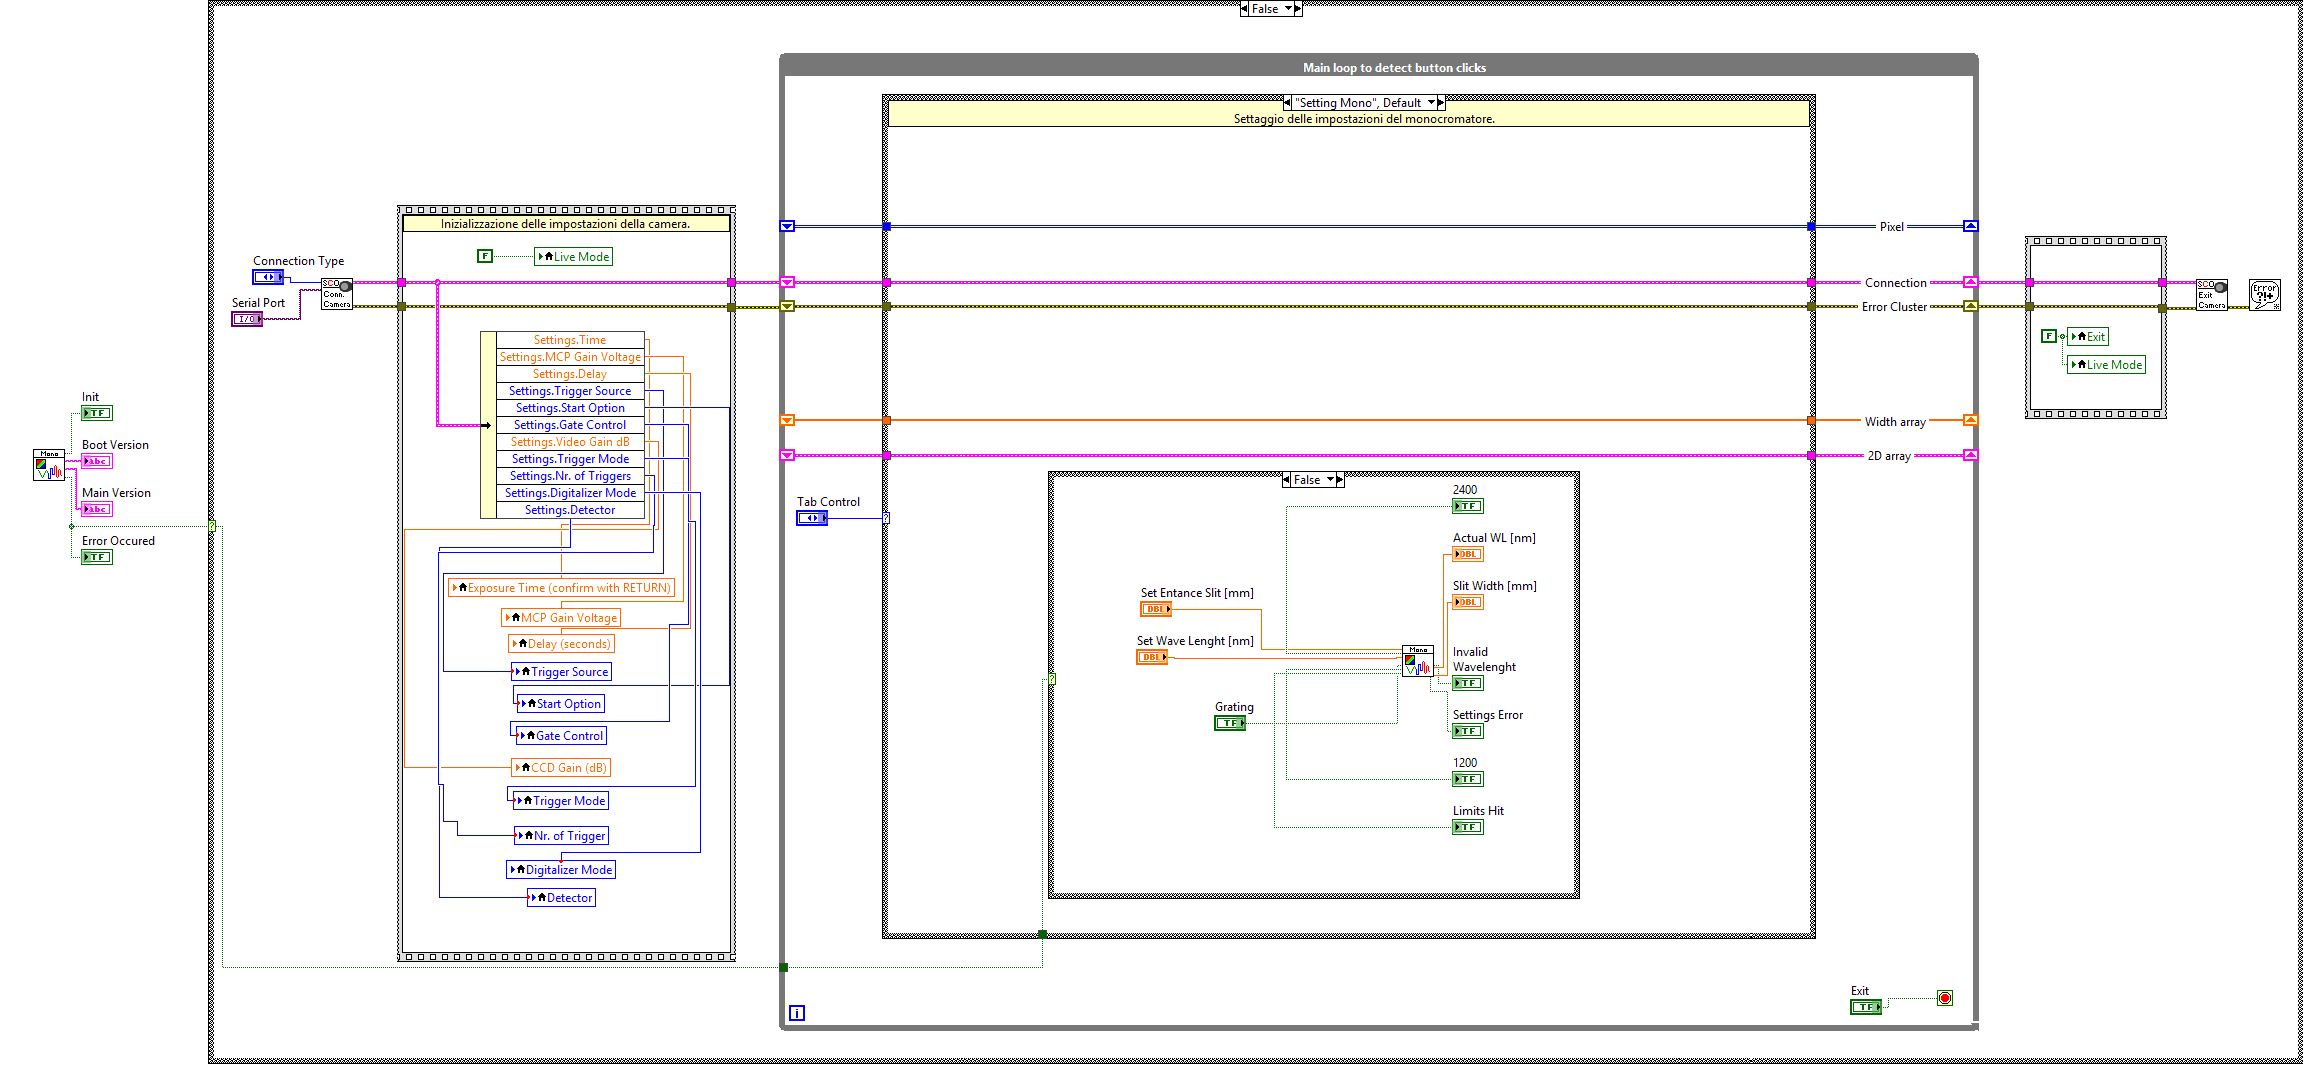
\includegraphics[width=\linewidth]{img/Main_bd.png}
	\caption{Block Diagram del progetto}
	\label{fig:newProj_bd}
\end{figure}
Come detto sopra il programma � stato organizzato in un progetto che raggruppa tutti i subVI creati nel corso della scrittura del codice. Partendo dal VI principale \emph{Main.vi} si descrive il block diagram delineando poi nello specifico i singoli subVI.\\
Il primo subVI che viene eseguito � \emph{InitMono.vi} che, come si pu� intuire dal nome, ha il compito di inizializzare il monocromatore; solo se tale subVI esegue restituendo nessun errore � possibile continuare con il resto del programma, del resto non avrebbe senso se lo strumento che deve generare il soggetto delle immagini non funziona correttamente. Se quindi non ci sono errori in fase di inizializzazione del monocromatore si entra in una case structure che racchiude tutto il resto del programma: per prima cosa viene eseguito il subVI di connessione alla fotocamera \emph{ConnectCamera.vi} il cui output entra poi in una flat sequence atta a visualizzare le impostazioni della fotocamera inserite l'ultima volta che � stata utilizzata. Successivamente si entra in un ciclo while per rilevare le azioni dell'utente; all'interno di questo ciclo si trova una case structure legata al \textit{tab control} che permette alla struttura di discriminare il codice in base alla tab selezionata dall'utente. La scelta di tale schema prende spunto dal design pattern di macchina a stati finiti: non � presente un enumerativo e non c'� una vera e propria sequenza che viene eseguita, ma lo schema generale ricorda tale pattern. Analizziamo quindi il codice eseguito nei quattro frame:
\begin{description}
\item[Setting Mono] Figura \ref{fig:newProj_bd}. All'interno di un'ulteriore case structure viene eseguito il subVI \emph{SettingMono.vi}.
\begin{figure} [h]
	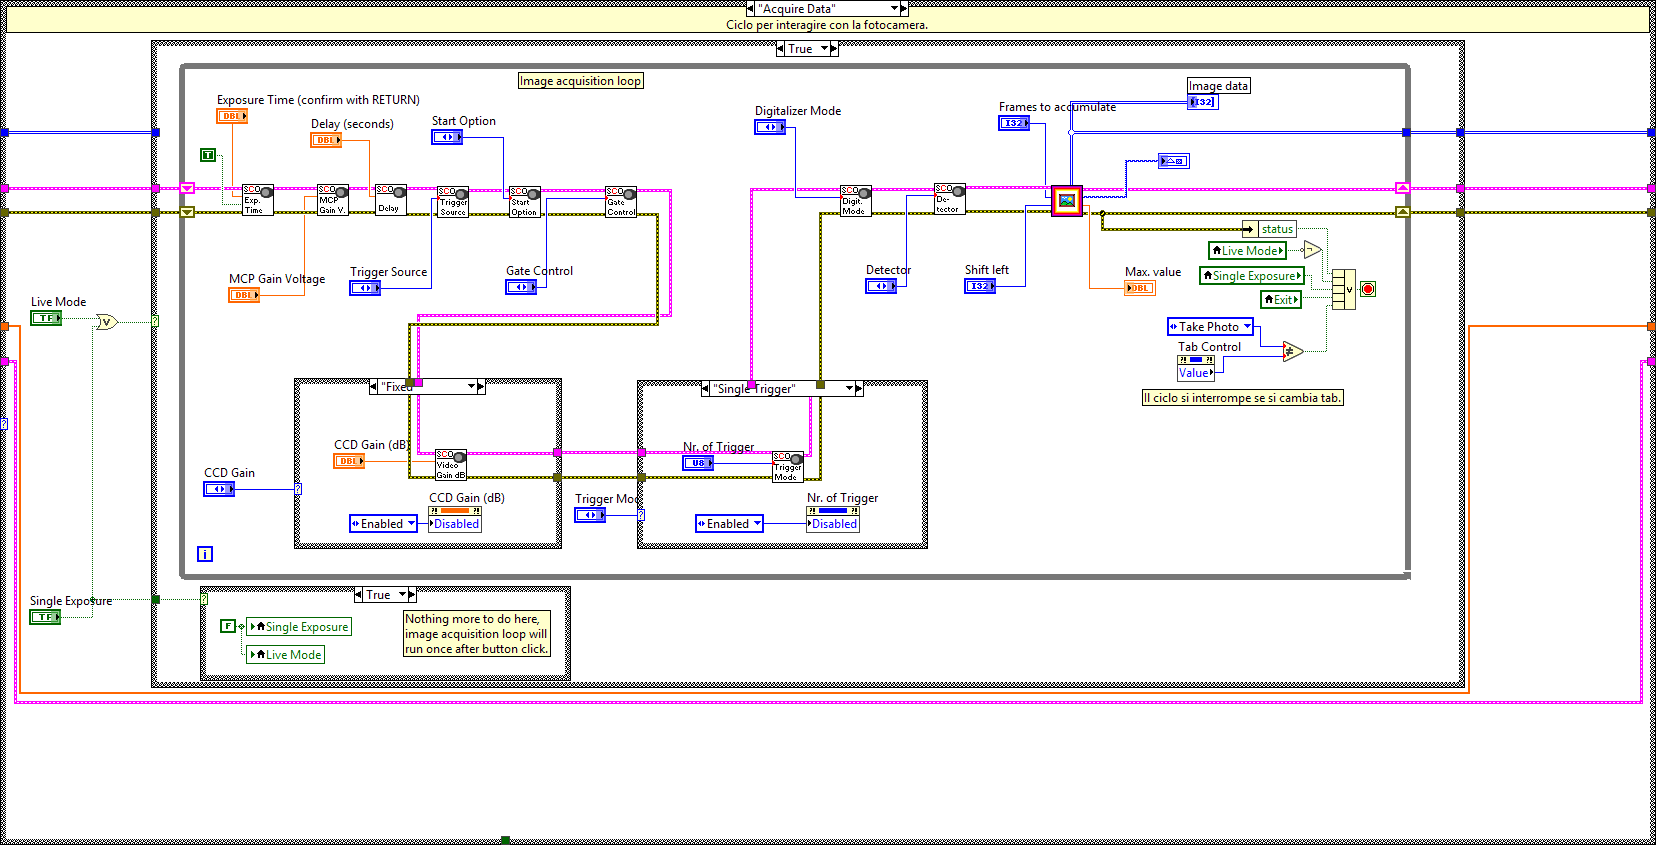
\includegraphics[width=\linewidth]{img/Main_acquireData.png}
	\caption{Block Diagram del progetto, frame ``Acquire Data''}
	\label{fig:newProj_bd_acquire}
\end{figure}
\item[Acquire Data] Figura \ref{fig:newProj_bd_acquire}. Per questa frame della case structure si � scelto di non creare subVI in quanto le variabili di input e output sarebbero state troppo numerose e avrebbero reso il codice incomprensibile. Viene quindi eseguito il codice per l'acquisizione delle immagini (si fa riferimento a quello spiegato nel capitolo precedente). Il ciclo per l'acquisizione viene arrestato anche se viene selezionata dall'utente un'altra tab.
\begin{figure} [h]
	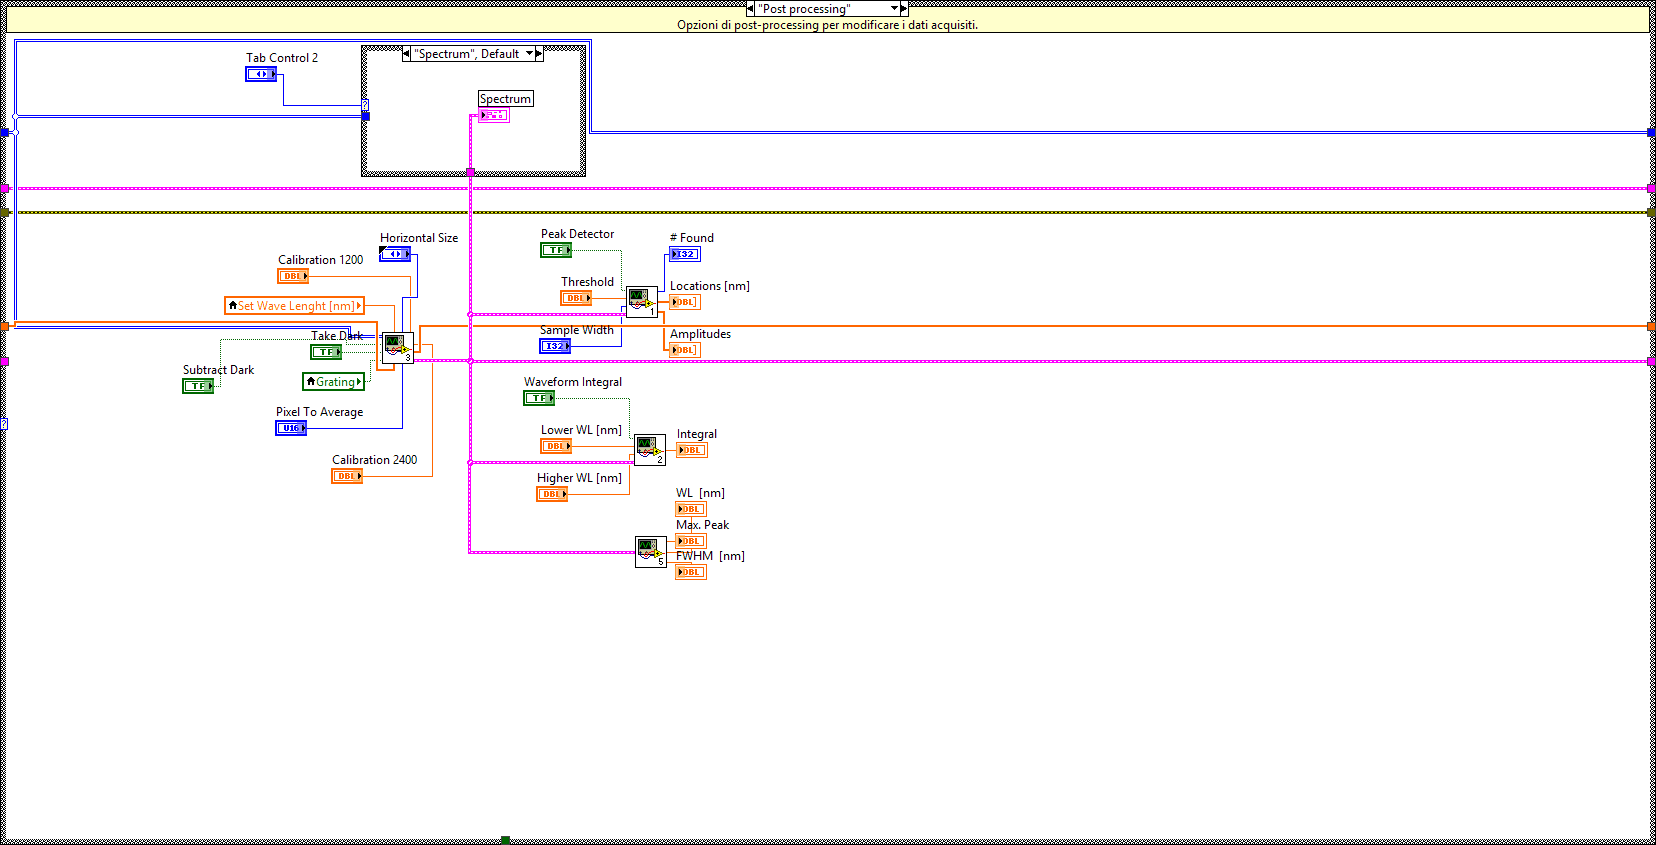
\includegraphics[width=\linewidth]{img/Main_postProc.png}
	\caption{Block Diagram del progetto, frame ``Post Processing''}
	\label{fig:newProj_bd_post}
\end{figure}
\item[Post processing] Figura \ref{fig:newProj_bd_post}. In questa frame sono stati inserite le elaborazioni sui dati che possono essere eseguite in seguito all'acquisizione dei dati. Abbiamo quindi una case structure che permette di visualizzare i dati come immagine o come spettro. Ci sono poi tre subVI: \emph{CreateSpectrum.vi} effettua i calcoli necessari per generare lo spettro da visualizzare, \emph{PeaksDetector.vi} restituisce i picchi sopra una certa soglia, \emph{FindWavefromIntegral.vi} calcola l'integrale su un intervallo della lunghezza d'onda.
\begin{figure} [h]
	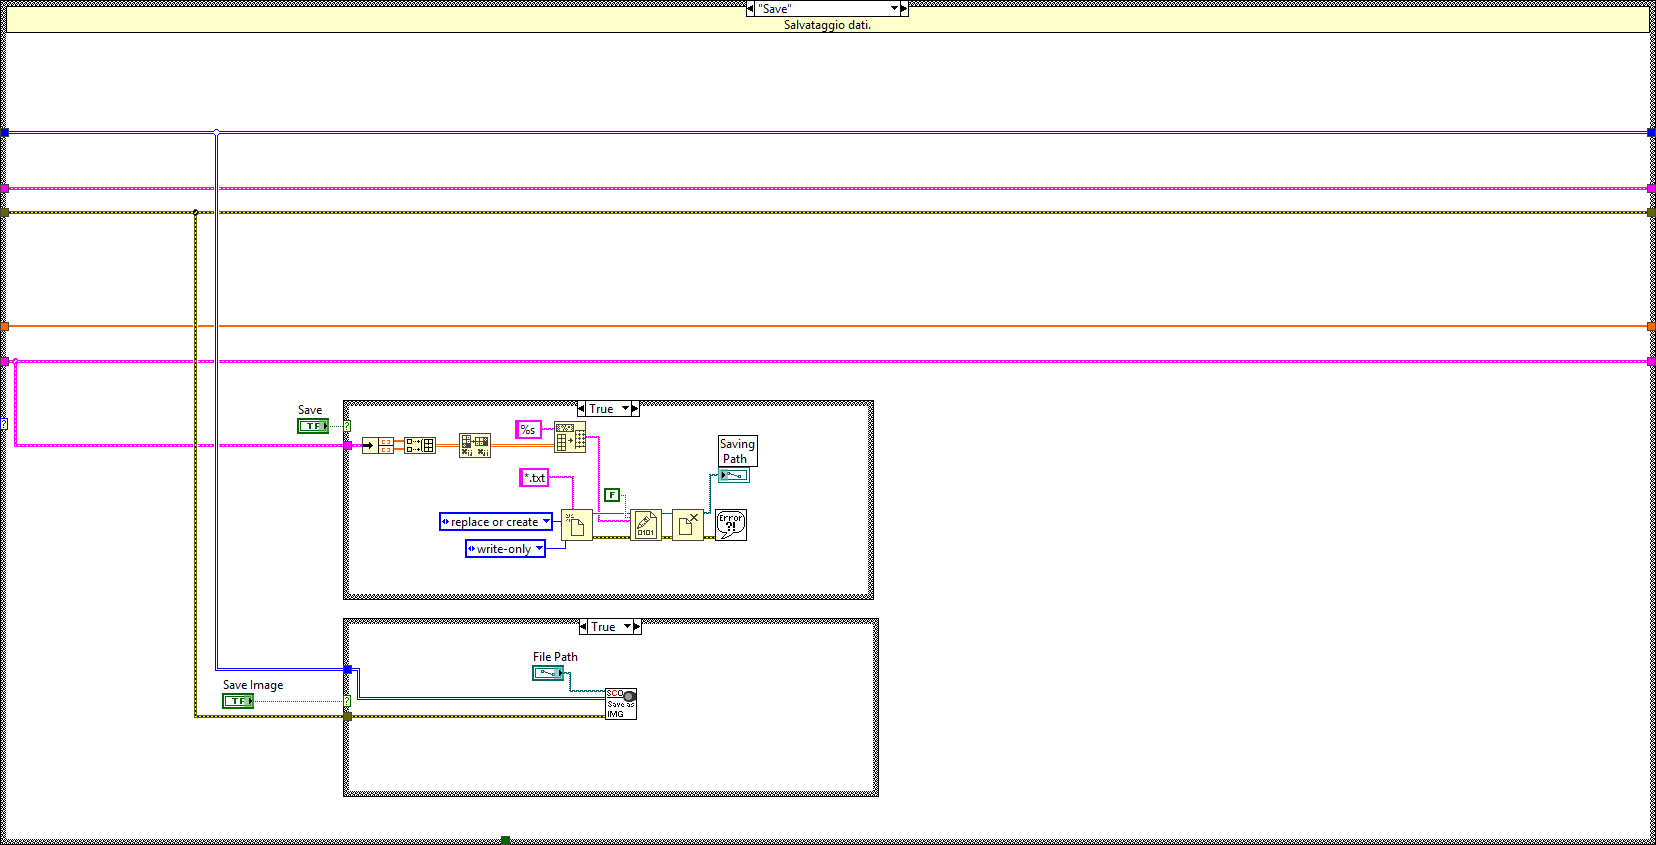
\includegraphics[width=\linewidth]{img/Main_save.png}
	\caption{Block Diagram del progetto, frame ``Save''}
	\label{fig:newProj_bd_save}
\end{figure}
\item[Save] Figura \ref{fig:newProj_bd_save}. Questa frame contiene due opzioni di salvataggio: \textit{Save} per salvare i dati in un file di testo, \textit{Save Image} per salvare l'immagine.
\end{description}
I shift register del ciclo esterno sono cinque: \textit{Pixel} contiene la matrice di pixel che compone l'immagine, \textit{Connection} contiene tutte le informazioni relative alla fotocamera, \textit{Error Cluster} riporta gli eventuali errori generati dalla fotocamera, \textit{Width Array} � l'array che contiene i valori delle lunghezze d'onda, \textit{2D Array} � la matrice con i valori da inserire nel grafico dello spettro.\\
Se infine viene arrestato il ciclo con il comando \textit{Exit}, viene eseguita l'ultima flat sequence che resetta i valori dei controlli di acquisizione delle immagini e viene eseguito anche il subVI \emph{ExitCamera.vi} per la chiusura graceful del programma e il rilascio delle risorse.

\subsection{Descrizione subVI}
Si descrivono di seguito i singoli subVI e le loro funzionalit�. Saranno analizzati solo i block diagram, in quanto i front panel hanno il solo scopo di mostrare input e output.
\begin{description}
\begin{figure} [h]
	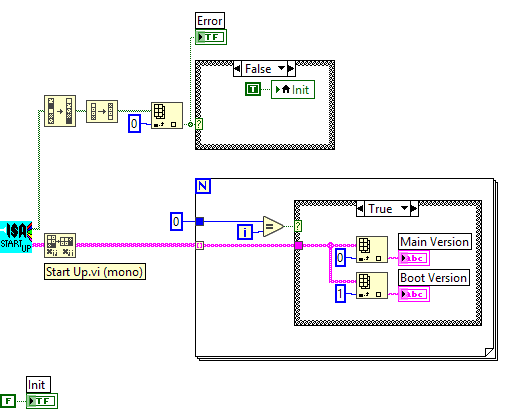
\includegraphics[width=\linewidth]{img/InitMonod.png}
	\caption{Block Diagram del subVI \emph{InitMono.vi}}
	\label{fig:newProj_bd_sub_initMono}
\end{figure}
\item[\textit{InitMono.vi}] Figura \ref{fig:newProj_bd_sub_initMono}. Il compito di questo subVI � quello di interrogare il monocromatore riportandolo al suo stato di default. Rispetto al codice presente nel progetto antecedente � stato leggermente modificato. Sono state eliminate tutte le flat sequence, che forzano il flusso logico dei dati. Dopo che � stato invocato il subVI del monocromatore \emph{Start Up.vi}, il led \textit{Init} viene impostato a true solo ed esclusivamente se non sono presenti errori nella matrice di errori restituita dallo stesso.
\begin{figure} [h]
	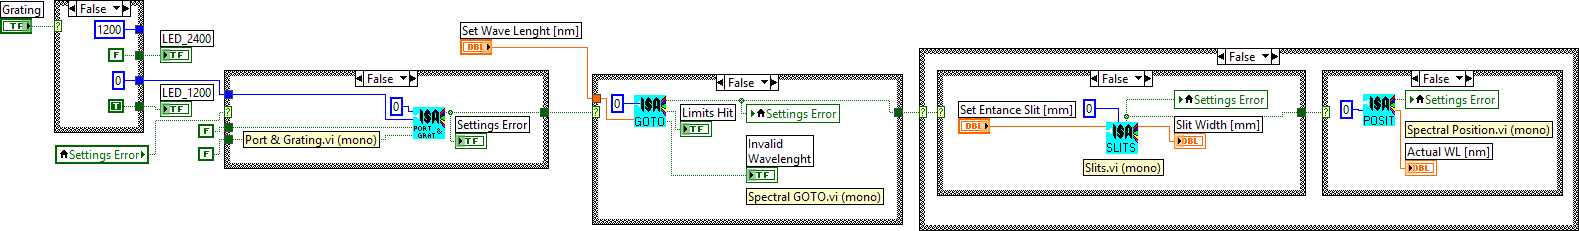
\includegraphics[width=\linewidth]{img/SettingMonod.png}
	\caption{Block Diagram del subVI \emph{SettingMono.vi}}
	\label{fig:newProj_bd_sub_settingMono}
\end{figure}
\item[\textit{SettingMono.vi}] Figura \ref{fig:newProj_bd_sub_settingMono}. Anche questo subVI � stato modificato rispetto al codice precedente eliminando tutte le flat sequence. La descrizione di tale subVI � la stessa illustrata \textbf{---METTERE RIFERIMENTO---}
\begin{figure} [h]
	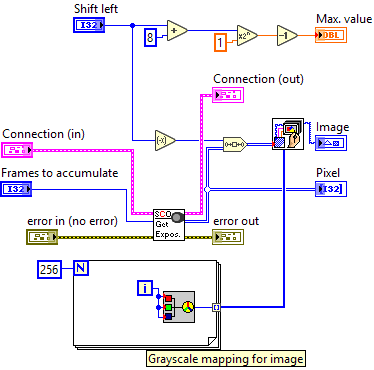
\includegraphics[width=\linewidth]{img/CreateImaged.png}
	\caption{Block Diagram del subVI \emph{CreateImage.vi}}
	\label{fig:newProj_bd_sub_CreateImage}
\end{figure}
\item[\textit{CreateImage.vi}] Figura \ref{fig:newProj_bd_sub_CreateImage}. In seguito all'invocazione del subVI della fotocamera \emph{GetExposure.vi} viene invocata la funzione \emph{Draw Unflattened Pixmap.vi} per creare l'immagine vera e propria che possa essere visualizzata in un indicatore apposito.
\begin{figure} [h]
	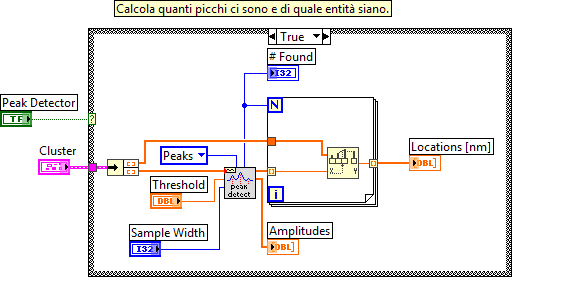
\includegraphics[width=\linewidth]{img/PeaksDetectord.png}
	\caption{Block Diagram del subVI \emph{PeaksDetector.vi}}
	\label{fig:newProj_bd_sub_PeaksDetector}
\end{figure}
\item[\textit{PeaksDetector.vi}] Figura \ref{fig:newProj_bd_sub_PeaksDetector}. Lo scopo di questo subVI � quello di trovare, attraverso la funzione \emph{Waveform Peak Detection.vi}, il numero di picchi presenti nella matrice in ingresso con rispettivi valori di lunghezza d'onda e intensit� del picco.
\begin{figure} [h]
	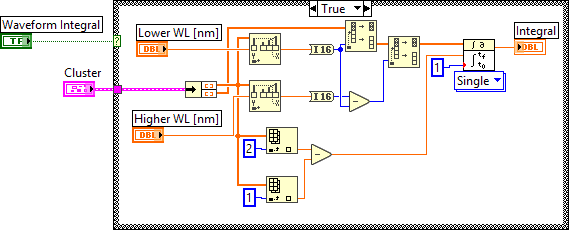
\includegraphics[width=\linewidth]{img/FindWaveformIntegrald.png}
	\caption{Block Diagram del subVI \emph{FindWaveformIntegral.vi}}
	\label{fig:newProj_bd_sub_FindWaveformIntegral}
\end{figure}
\item[\textit{FindWavefromIntegral.vi}] Figura \ref{fig:newProj_bd_sub_FindWaveformIntegral}. Data in ingresso la matrice con lunghezza d'onda e intensit� dello spettro, questo subVI calcola l'integrale, con apposite funzioni, su un intervallo in input.
\begin{figure} [h]
	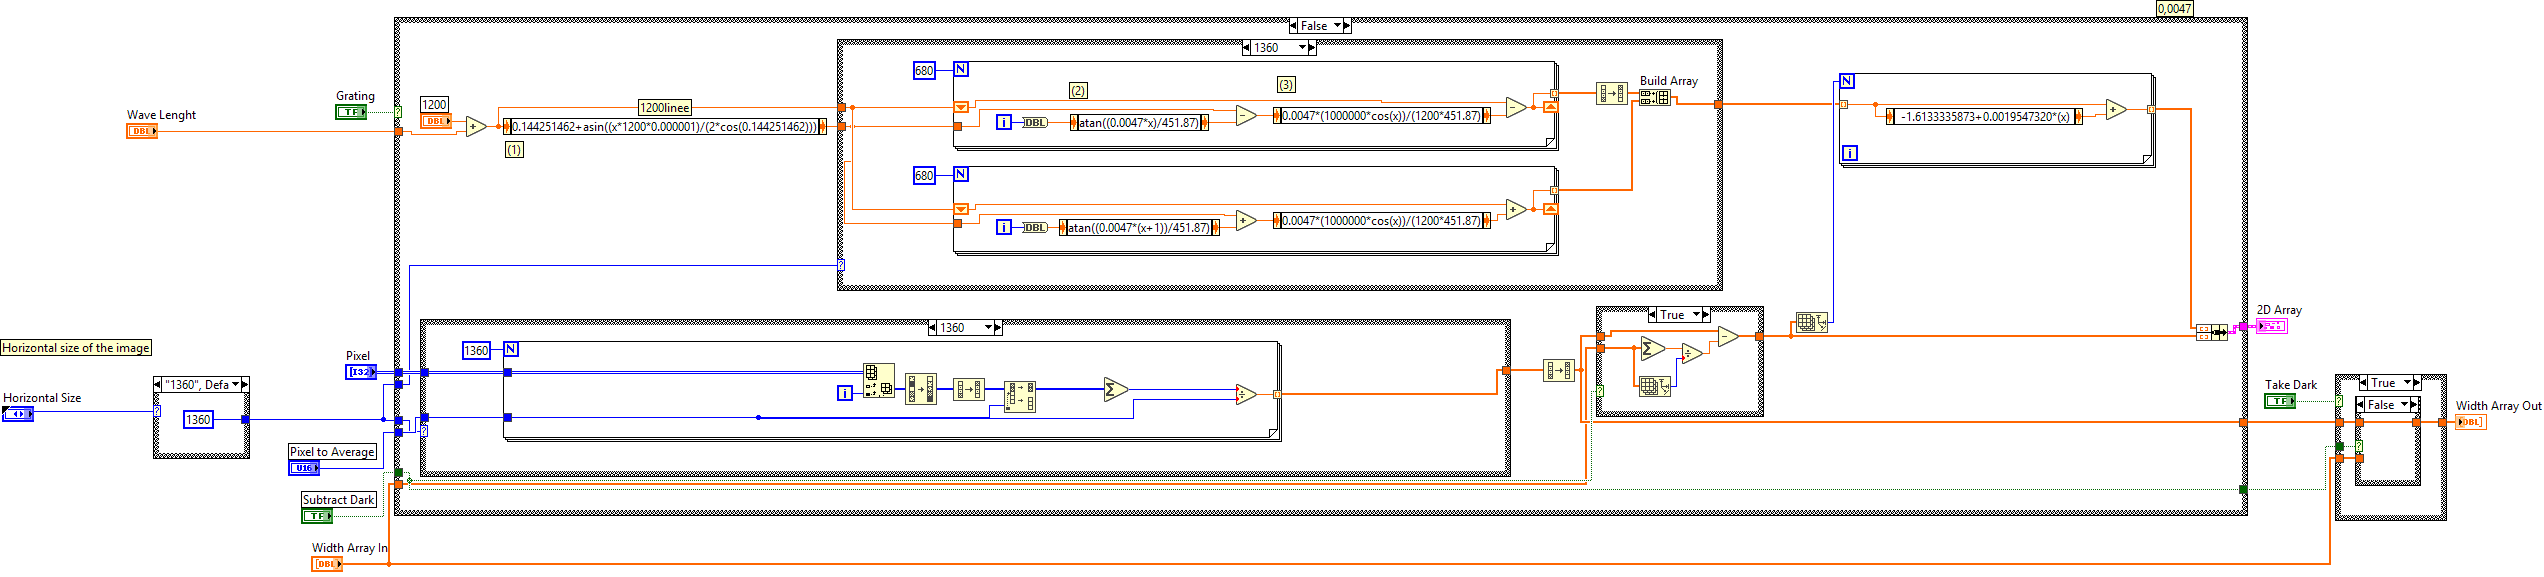
\includegraphics[width=\linewidth]{img/CreateSpectrumd.png}
	\caption{Block Diagram del subVI \emph{CreateSpectrum.vi}}
	\label{fig:newProj_bd_sub_CreateSpectrum}
\end{figure}
\item[\textit{CreateSpectrum.vi}] Figura \ref{fig:newProj_bd_sub_CreateSpectrum}. Come si pu� intuire dal nome, l'output di questo subVI consiste in una matrice di valori che rappresentano lunghezze d'onda con rispettiva intensit� dello spettro. I calcoli presenti sono stati riportati dal progetto precedente in quanto legati al monocromatore. � stato modificato il valore del numero di pixel della larghezza dell'immagine (1360) e il valore di pixel/nm (0.0047) (???).
\begin{figure} [h]
	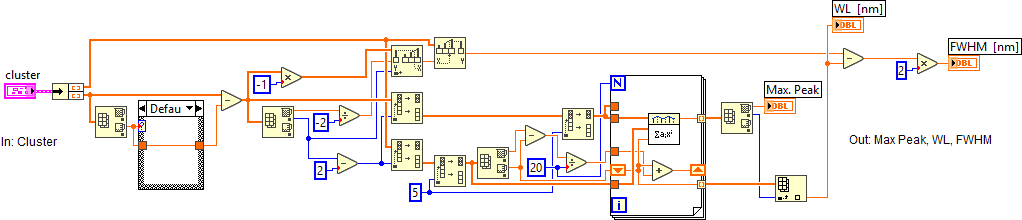
\includegraphics[width=\linewidth]{img/FindMaxPeakWLFWHMd.png}
	\caption{Block Diagram del subVI \emph{FindMaxPeak\&WL\&FWHM.vi}}
	\label{fig:newProj_bd_sub_FindMaxPeakWLFWHM}
\end{figure}
\item[\textit{FindMaxPeak\&WL\&FWHM.vi}] Figura \ref{fig:newProj_bd_sub_FindMaxPeakWLFWHM}. Questo subVI produce due risultati: restituisce il picco massimo e la sua corrispettiva lunghezza d'onda, e il valore della FWHM (Full Width at Half Maximum).
\end{description}
\begin{figure} [h]
	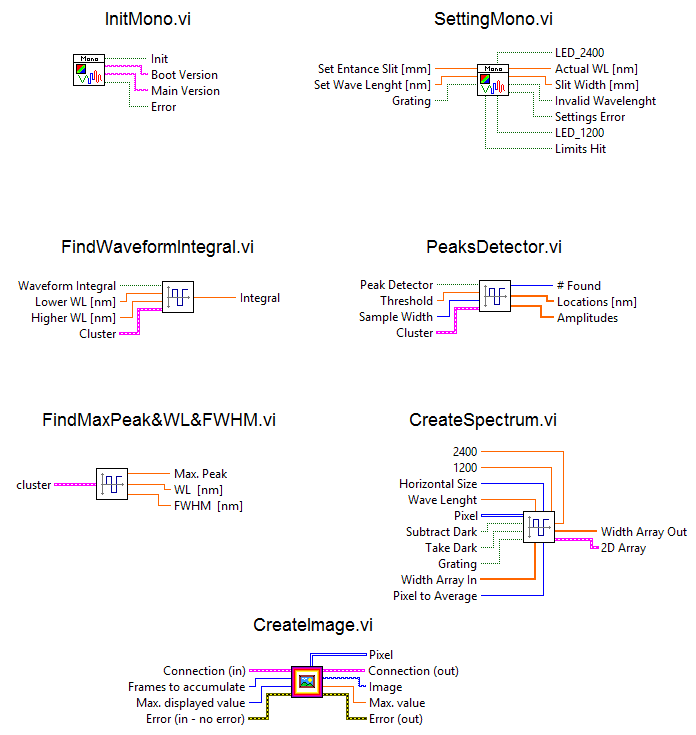
\includegraphics[width=\linewidth]{img/IconeSubVI.png}
	\caption{Icone dei subVI del progetto}
	\label{fig:newProj_bd_sub_icons}
\end{figure}
Nella figura \ref{fig:newProj_bd_sub_icons} si possono vedere le icone con input e output di tutti i subVI citati.